% --------------------------------------------------------------------------- %
% TDT4215 Web-intelligence - Group project
% NTNU spring 2013
%
% Anders Palfi
% Javier Elizaga Quevedo
% Einar Uvsløkk
% --------------------------------------------------------------------------- %

\documentclass[11pt,a4paper]{report}
\usepackage[utf8]{inputenc}
\usepackage[english]{babel}
\usepackage[pdftex]{graphicx}
\usepackage{color}
\usepackage{mathtools}
\usepackage[intoc]{nomencl}
\usepackage{booktabs}
\usepackage{hyperref}


\setcounter{tocdepth}{1}
\makenomenclature


% --------------------------------------------------------------------------- %
% Definitions
% --------------------------------------------------------------------------- %
\definecolor{darkred}{rgb}{.5,0,0}
\definecolor{darkgreen}{rgb}{0,.5,0}
\definecolor{darkblue}{rgb}{0,0,.5}
\hypersetup{
	colorlinks,
	linkcolor=darkblue,
	filecolor=darkgreen,
	urlcolor=darkred,
	citecolor=darkblue}


% --------------------------------------------------------------------------- %
% Custom commands
% --------------------------------------------------------------------------- %
\newcommand{\ICD}{International Classification of Diseases}
\newcommand{\ATC}{Anatomical Therapeutic Chemical classification of Drug}
\newcommand{\HRule}{\rule{\linewidth}{0.5mm}}
\newcommand{\opn}{\operatorname}


\begin{document}


% --------------------------------------------------------------------------- %
% Title page
% --------------------------------------------------------------------------- %
\begin{titlepage}
\center
\textsc{\Large Norwegian University of Science and Technology}\\[1.5cm]
\textsc{\large Department of Computer and Information Science}\\[0.5cm]
\textsc{TDT4215 Web-intelligence}\\[0.5cm]

\HRule \\[0.5cm]
{\huge \bfseries Project report}\\[0.2cm]
\HRule \\[1.5cm]

\Large \emph{Authors:}\\
Anders \textsc{Palfi}\\
Javier \textsc{Elizaga Quevedo}\\
Einar \textsc{Uvsløkk}\\[3cm]

{\large Word count: 1146}\\
{\large \today}\\[3cm]

\vfill

\end{titlepage}


% --------------------------------------------------------------------------- %
% Table of contents
% --------------------------------------------------------------------------- %
\tableofcontents
\renewcommand{\nomname}{List of Abbreviations}
\printnomenclature

\nomenclature{API}{Application programming interface}
\nomenclature{ATC}{Anatomical Therapeutic Chemical classification of Drug}
\nomenclature{HTML}{HyperText Markup Language}
\nomenclature{ICD}{International Classification of Diseases}
\nomenclature{OWL}{Web Ontology Language}
\nomenclature{VSM}{Vector Space Model}
\nomenclature{XML}{Extensible Markup Language}

% vim: set ts=2 sw=2 tw=80:

\listoffigures
\addcontentsline{toc}{chapter}{List of Figures}


% --------------------------------------------------------------------------- %
% Chapters
% --------------------------------------------------------------------------- %
\chapter{Introduction} \label{cha:Introduction}

This paper documents our work with the group project in TDT4215
Web-intelligence, at Norwegian University of Science and Technology (NTNU).

The project assignment is to design and implement a search system that uses
patient record notes as a search query to chapters of the Norwegian electronic
handbook for pharmaceutical interventions
(Legemiddelhåndboka)\cite{website:nlh}.

\chapter{Method}
\label{cha:method}


% --------------------------------------------------------------------------- %
% Preprocessing
% --------------------------------------------------------------------------- %
\section{Preprocessing}
\label{sec:preprocessing}

We started with parsing Legemiddelhåndboka. We parsed page at a time and created
a Chapter java object of each chapter. If a chapter contains sub-chapters they
will be saved in a list of chapter objects in the parents’ chapter object. We
made custom parser using the Jsoup library. When we had parsed and made java
objects of all the chapters we used stored these objects for later use using
JSON format. This is because parsing the Legemiddelhåndboka takes some time and
does not need to be done every time the system starts. We chose JSON format
because this is readable for humans which was handy during development.

We first parse the OWL files using the OWL API. The information we got from each
class in the OWL ontology we saved as serializable Java objects. The Java
objects have a String field for each annotation of each class of the OWL
ontology.

We decided not to preprocess any of the cases. This is because they were small
and easy to parse. We just copied the files from the docx file and created a
.txt file for each case.

For all the text we parsed we removed all non-alphabetic characters. This was
because we did not think those characters provides us with any valuable
information.

After this step we got all the necessary information from Legemiddelhåndboka chapters
and the text (from annotations) from the owl classes saved in java objects.


% --------------------------------------------------------------------------- %
% ICD-10 codes
% --------------------------------------------------------------------------- %
\section{ICD-10-codes}
\label{sec:}

We use Lucene as a search engine for matching similarities between the ICD-10
ontology and the patient cases. What we did was to create and index Lucene
documents, this documents has two main fields; a Lucene TextField with the
description of each class (label, underterm, synonym annotations) and a Lucene
StringField with the ICD-10 code. Lucene will only tokenize the TextField
content.

For each sentence in each chapter in Legemiddelhåndboka we used the index we
created to get the Lucene document(that contains the information from the the
owl class) that had the best score. From this document we retrieved the ICD-10
code. When we got all the ICD-10 codes for every sentence in each chapter we
updated the JSON file to also contain these codes, since these won’t ever change
as long as the text in Legemiddelhåndboka doesn’t change.

We found the ICD-10 code that matched each sentence in each of the patient cases
as well, but we did not bother storing these as this job is lightweight compared
to getting the ICD-10 codes for all the Legemiddelhåndboka chapters.

After this step we got a string of ICD-10 codes for every chapter and all the
patient cases.


% --------------------------------------------------------------------------- %
% Ranking
% --------------------------------------------------------------------------- %
\section{Ranking}
\label{sec:ranking}

Since we got ICD-10 codes for each chapter as well as ICD-10 codes for each
patient case we had to use these to get the most relevant chapter for each
patient case. The way we approached it was to create an Lucene index with all
the ICD-10 codes from each chapter. Then we query this index with the ICD-10
codes for each patient as a query string. The thought behind this is that if a
ICD-10 codes is relevant for many sentences in a Legemiddelhåndboka chapter as
well as relevant for many sentences in a patient case, then the chapter and the
case is most likely relevant to each other.


% vim: set ts=2 sw=2 tw=80

\chapter{System architecture}
\label{cha:architecture}

This section describes the system architecture of our solution.


% --------------------------------------------------------------------------- %
% Components
% --------------------------------------------------------------------------- %
\section{Components}
\label{sec:components}

Figure \ref{fig:class-diagram} show the structure of the components.

\begin{figure}
\begin{center}
	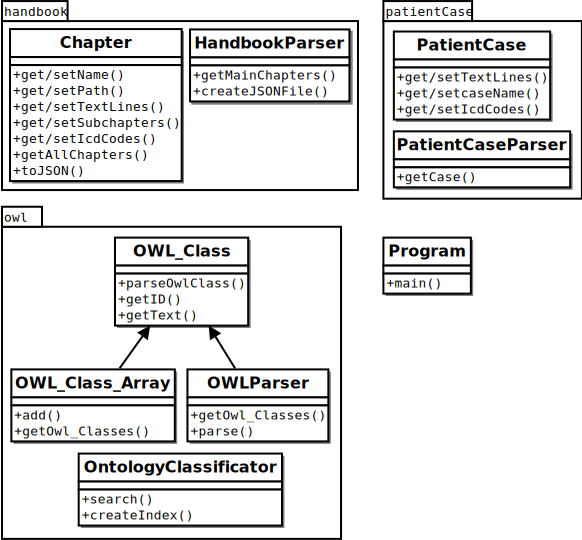
\includegraphics[width=\textwidth]{figures/class-diagram}
\end{center}
\caption{Class diagram}
\label{fig:class-diagram}
\end{figure}


% --------------------------------------------------------------------------- %
% External libraries
% --------------------------------------------------------------------------- %
\section{External libraries}
\label{sec:external-libraries}

\subsection*{Jsoup}
Jsoup is an open source java library for working with real-world HTML. It
provides a very convenient API for extracting and manipulating data. We use
Jsoup during the parsing of Legemiddelhåndboka.\\\\
\url{http://jsoup.org/}

\subsection*{The OWL API}
The OWL API is an open source java library used when working with owl
ontologies. We use this api when we’re retrieving information from the icd-10
owl ontology.\\\\
\url{http://owlapi.sourceforge.net/}

\subsection*{JSON.simple}
JSON simple is a java toolkit that are used to encode/decode JSON text. We use
this to when we want to save the chapters of Legemiddelhåndboka. We chose
JSON.simple because it provides a very simple and basic tool to convert java
objects to JSON text, which is just what we needed.\\\\
\url{https://code.google.com/p/json-simple/}

\subsection*{Lucene}
Apache Lucene is an open source text search engine library written in Java. We
use Lucene for all our indexing/searching operation in our solution.\\\\
\url{http://lucene.apache.org/core/}

% vim: set ts=2 sw=2 tw=80:

\chapter{Theory}
\label{cha:theory}

% --------------------------------------------------------------------------- %
% Indexing
% --------------------------------------------------------------------------- %
\section{Indexing}
\label{sec:indexing}

Lucene work with Document objects, each Document have Fields, each Field is
analyzed differently, for instance: a TextField is for content we want tokenized
(the description part of the icd10 codes), and StringField is for content we
don't want tokenized (the icd10 codes).

There are two main parts in the indexing process:

\begin{itemize}
\item The Analyzer extracts tokens out of text to be indexed.

\item The IndexWriter is a key component in the indexing process, is the one
      that adds documents to the index.
\end{itemize}


% --------------------------------------------------------------------------- %
% Scoring
% --------------------------------------------------------------------------- %
% TODO typeset math equations
\section{Scoring}
\label{sec:scoring}

The documents are chosen by a Boolean Model and are scored by a Vector Space
Model (VSM).
% TODO abbr ref VSM
\[
	\operatorname{cosine-similarity}(q,d) = \frac{V(q) \cdot V(d)} {|V(q)|\ |V(d)|}
\]
%
Where \(V(q) \cdot V(d)\) is the dot product (intersection) of the weighted
vectors, and \(|V(q)|\) and \(|V(d)|\) are their Euclidean norms.\\
\\
For practical reasons the real formula that Lucene uses is:
%
\begin{equation*}
\begin{split}
	\operatorname{score}(q,d) =
	& \operatorname{coord}(q,d) \cdot
		\operatorname{queryNorm}(q)  \\
	& \cdot
		\sum_{t \operatorname{in} q} (
			\operatorname{tf}(t\operatorname{in}d) \cdot
			\operatorname{idf}(t)^{2} \cdot
			\operatorname{t.getBoost}() \cdot
			\operatorname{norm}(t,d)
		)
\end{split}
\end{equation*}
%
\begin{description}

\item[\(tf(t\operatorname{in}d)\)]
correlates to the term's frequency, defined as the number of times term \(t\)
appears in the currently scored document \(d\).

\item[\(\operatorname{idf}(t)\)]
stands for Inverse Document Frequency.
\[
	\operatorname{idf}(t) = 1 + \log(\frac{numDocs}{docFreq + 1})
\]

\item[\(\operatorname{coord}(q,d)\)]
is a score factor based on how many of the query terms are found in the
specified document.

\item[\(\operatorname{queryNorm}(q)\)]
is a normalizing factor, doesn’t affect to the ranking.

\item[\(\operatorname{t.getBoost}()\)]
is a search time boost of term t in the query q.

\item[\(\operatorname{norm}(t,d)\)]
encapsulates a few (indexing time) boost and length factors.

\end{description}

% vim: set ts=2 sw=2 tw=80:

\chapter{Result}
\label{cha:result}

\ldots


\chapter{Conclusion}
\label{cha:conclusion}

\ldots



% --------------------------------------------------------------------------- %
% Bibliography
% --------------------------------------------------------------------------- %
\bibliographystyle{alpha}
\bibliography{bibliography}
\addcontentsline{toc}{chapter}{Bibliography}


% --------------------------------------------------------------------------- %
% Appendices
% --------------------------------------------------------------------------- %


\end{document}

% vim: set ts=2 sw=2 tw=80:
